\section{Signal to Noise Ratio}

%---------------------------------------------------------

\begin{frame}
    \frametitle{Signal-to-Noise Ratio (SNR): Introduction and Definition}
    \begin{block}{What is SNR?}
        \begin{itemize}
            \item Standalone metric, it can be obtained directly from side-channel traces without needing to launch a full attack
            \item Provides a quick assessment of the quality of information leakage present in the measurements
        \end{itemize}
    \end{block}

    \begin{block}{}
        \begin{itemize}
            \item SNR quantifies the ratio between the strength of the "signal" $L_d$(the useful, data-dependent part of the leakage) and the strength of the "noise" $L_n$ (the random, useless part) \newline \newline
                    $$L=L_d+L_n=g(V)+L_n$$ \text{        where        } $L_n \sim N (0, \sigma^2 )$.

            \item A higher SNR indicates stronger and clearer leakage, making it potentially easier to exploit
        \end{itemize}
    \end{block}
\end{frame}
\begin{frame}
    \frametitle{Signal-to-Noise Ratio (SNR): Introduction and Definition}
    \begin{block}{Mathematical Definition}
            Formally, SNR is defined as the ratio of the variance of the deterministic leakage to the variance of the noise:
            $$ \text{SNR} = \frac{\text{Var}(L_d)}{\text{Var}(L_n)} $$
    \end{block}
\end{frame}


\begin{frame}
\frametitle{SNR: Understanding and Utilizing Leakage}
    \begin{block}{Interpreting SNR}
        \begin{itemize}
            \item A high SNR indicates that the signal component dominates the noise, suggesting clear leakage points
            \item Helps in identifying the most promising Points of Interest (POIs) within a trace, where the leakage is strongest
            \item Can be used to compare the leakage characteristics of different implementations or countermeasures
        \end{itemize}
    \end{block}
\end{frame}







%---------------------------------------------------------

\begin{frame}
    \frametitle{Computing SNR with Simulated Leakage}
    
            In this scenario, the attacker explicitly simulates the leakage $L$ \newline
            This is done by precisely defining its deterministic part ($L_d$) and its noise component ($L_n$)
   

    \begin{block}{Example: 8-bit Value Leakage}
        \begin{itemize}
            \item Simulate the leakage of an 8-bit value $V$ (uniformly random)
            \item Choose a leakage function $g(V) = \alpha V + \beta$, where $\alpha, \beta$ are known constants
            \item Thus, $L_d = \alpha V + \beta$, representing a scaled and offset version of identity leakage
            \item Choose noise $L_n \sim \mathcal{N}(0, \sigma^2)$, specifying $\sigma^2$
            \item The simulation can be noiseless ($\sigma = 0$) to identify leakage, or noisy ($\sigma \ne 0$) to analyze device/countermeasure behavior in the presence of noise
        \end{itemize}
    \end{block}
\end{frame}


\begin{frame}
    \frametitle{SNR with Simulated Leakage: Computation}
    
            In this controlled simulation, we can proceed to compute the SNR directly using the expectations $E(\cdot)$
       

    \begin{block}{Expectations of Deterministic Leakage}
        \begin{itemize}
            \item Expected value of $L_d$:
            $$ E(L_d) = E(g(V)) = \sum_{v=0}^{255} g(v)Pr(v) = \frac{1}{256} \sum_{v=0}^{255} (\alpha v + \beta) $$
            \item Expected value of $L_d^2$:
            $$ E(L_d^2) = E(g(V)^2) = \frac{1}{256} \sum_{v=0}^{255} (\alpha v + \beta)^2 $$
            \item $$ \text{SNR} = \frac{\text{Var}(L_d)}{\text{Var}(L_n)} = \frac{E(L_d^2) - E(L_d)^2}{\sigma^2} $$

        \end{itemize}
    \end{block}
\end{frame}

\begin{frame}
    \frametitle{SNR with Real Measurements}
    \begin{block}{}
        \begin{itemize}
            \item In a real-world scenario, we cannot directly observe the deterministic leakage ($L_d$) or the noise ($L_n$). We can only measure their sum, the total leakage ($L$).
            \item Our goal is to estimate the SNR from these real measurements without prior knowledge of the leakage function.
        \end{itemize}
    \end{block}
        Let's consider once again an example in which the leakage $L$ of an 8-bit value $V$ is observed, obtaining $n$ traces $l_1, ..., l_n$, each trace $l_i$ containing a single time sample that leaks information about $V$
\end{frame}
\newcommand{\Lagr}{\mathop{\mathcal{L}}}
\begin{frame}
    \begin{block}{Estimation Steps}
        \begin{itemize}
            \item 1. Partition traces: Group traces based on the value of the intermediate V (e.g., 256 groups for an 8-bit value). This way we obtain $\Lagr_0,\Lagr_1,...,\Lagr_{255}$. The set $\Lagr_v$ contains all traces $l$ that are observed when $V=v$
            \item 2. Estimate Means: Compute the mean trace $\hat{\mu}_v$ for each $\Lagr_v$ and the overall mean $\hat{\mu}$ . $$\hat{\mu}_v=\frac{1}{|\Lagr_v|}\sum_{l \in \Lagr_v} l$$ $$\hat{\mu}=\frac{1}{256}\sum_{v=0}^{255}\hat{\mu}_v$$ where $|\Lagr-v|$ is the number of traces for the group
        \end{itemize}
    \end{block}
\end{frame}

\begin{frame}
    \begin{block}{}
        \begin{itemize}
            \item 3. Estimate Variances: Compute the variance ($\hat{\sigma}_v^2$) for each group and the average of these variances ($\sigma^2$) as the noise variance.
            $$\hat{\sigma_v^2} = \frac{1}{|\Lagr_v|-1}\sum_{l \in \Lagr_v} (l-\hat{\mu_v})^2$$
            $$\hat{\sigma}^2=\frac{1}{256}\sum_{v=0}^{255}\hat{\sigma}_v$$
            \item 4. Compute SNR: The signal variance is the variance of the group means, while the noise variance is the average of the group variances. The SNR is their ratio.
                $$
                \text{SNR} = \frac{\text{Var}(L_d)}{\text{Var}(L_n)} = \frac{\sum_{v=0}^{255}(\hat{\mu}_v - \hat{\mu})^2}{\hat{\sigma}^2}
                $$
        \end{itemize}
    \end{block}
\end{frame}



%---------------------------------------------------------

\begin{frame}
    \frametitle{Interpreting an SNR Plot}
    \begin{block}{Example: Unprotected AES S-box}
        \begin{itemize}
            \item An SNR plot over time reveals when and where the most significant leakage occurs in an operation.
            \item High peaks in the plot correspond to specific time samples where the leakage is strongly correlated with the secret key.
            \item For instance, an unprotected AES S-box implementation on a Cortex-M0 microcontroller shows distinct peaks where key-dependent operations are performed, with an SNR of approximately 0.02.
            \item The overall shape of the SNR plot provides an overview of the inherent leakage of the device for a given implementation.
        \end{itemize}
    \end{block}
\end{frame}
\begin{frame}
\frametitle{}
    \begin{figure}
        \centering
        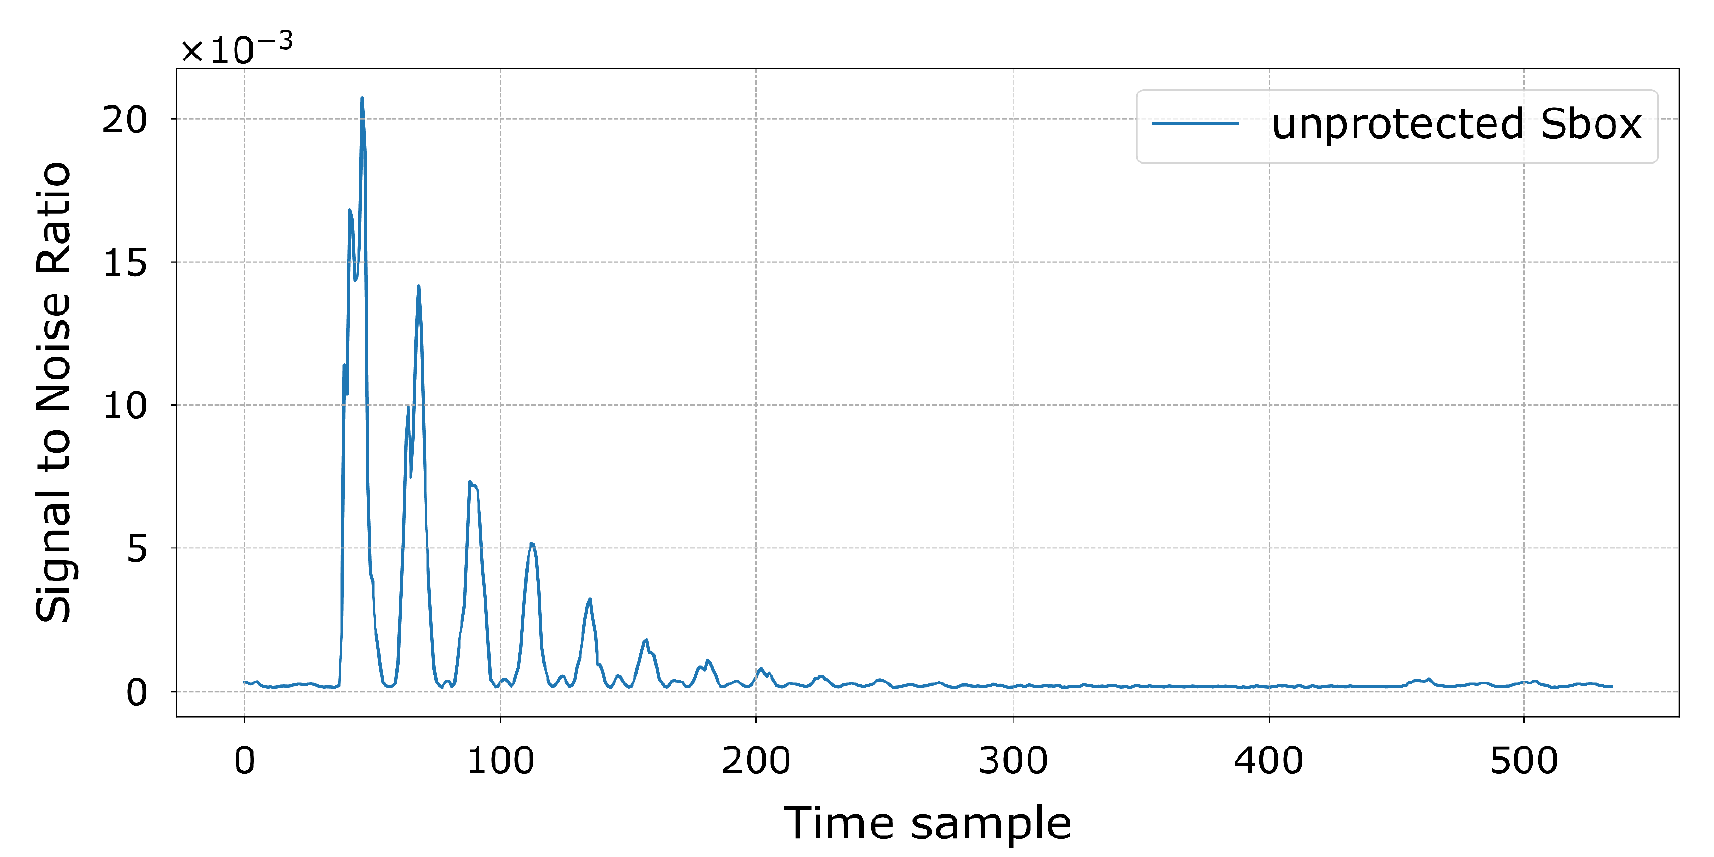
\includegraphics[width=1.0\textwidth]{metrics/Pictures/SNR_plot_unprotected_Sbox.png}
        \caption{SNR plot for an unprotected AES S-box implementation. Peaks indicate key-dependent leakage.}
    \end{figure}
\end{frame}



% Advantages and Limitations
\begin{frame}
    \frametitle{SNR: Limitations}
        \begin{itemize}
            \item \textbf{Not a direct attack feasibility metric:} It maintains a level of generality by not being tied to a specific attack method, but this also means it can't directly convey the actual security level of a device.
            \item \textbf{Simplified leakage model:} The metric implicitly relies on a simplified model of leakage (e.g., assuming a Gaussian noise distribution). In real-world scenarios, the actual leakage may diverge from these assumptions.
            \item \textbf{Parameter estimation issues:} The statistical parameters (mean and variance) must be adequately estimated from the available traces. A poor estimation due to a limited N.O.T. can lead to misleading SNR results.
            \item \textbf{Univariate nature:} The standard definition of SNR focuses on a single time sample at a time (univariate), ignoring the joint multivariate leakage that an adversary can exploit across multiple samples. 
        \end{itemize}
\end{frame}

